\documentclass[11pt,a4paper,oneside,openany,numbers=noendperiod]{scrreprt}

\usepackage[provide=*,spanish]{babel}
\usepackage{fontspec}
\setmainfont{Latin Modern Roman}
\setsansfont{Latin Modern Sans}
\setmonofont{Latin Modern Mono}[Scale=0.88,BoldFont={Latin Modern Mono}]
\usepackage{geometry}
\geometry{top=24mm,bottom=25mm,left=25mm,right=23mm,headsep=7mm,footskip=12mm}
\usepackage{microtype}
\usepackage{graphicx}
\graphicspath{{../docs/assets/}}
\usepackage{booktabs,longtable,tabularx,array,multirow}
\usepackage{ragged2e}
\usepackage{enumitem}
\usepackage{xcolor}
\usepackage{listings}
\usepackage{etoolbox,needspace,xurl}
\usepackage[most]{tcolorbox}
\usepackage{caption,subcaption}
\usepackage{float}
\usepackage{scrhack}
\usepackage{amsmath,amssymb}
\usepackage{csquotes}
\usepackage{scrlayer-scrpage}
\usepackage{hyperref}
\usepackage[capitalise,noabbrev,nameinlink]{cleveref}

\crefname{chapter}{capítulo}{capítulos}
\Crefname{chapter}{Capítulo}{Capítulos}
\crefname{section}{sección}{secciones}
\Crefname{section}{Sección}{Secciones}
\crefname{subsection}{sección}{secciones}
\Crefname{subsection}{Sección}{Secciones}
\crefname{table}{cuadro}{cuadros}
\Crefname{table}{Cuadro}{Cuadros}
\crefname{figure}{figura}{figuras}
\Crefname{figure}{Figura}{Figuras}

\definecolor{AkidaBlue}{HTML}{153B5B}
\definecolor{AkidaCyan}{HTML}{007F8B}
\definecolor{AkidaGreen}{HTML}{2C7A62}
\definecolor{AkidaAmber}{HTML}{A86400}
\definecolor{AkidaRed}{HTML}{A23832}
\definecolor{AkidaInk}{HTML}{1E2933}
\definecolor{AkidaPale}{HTML}{F3F7F8}
\definecolor{CodeBG}{HTML}{F5F6F7}

\hypersetup{
  colorlinks=true,
  linkcolor=AkidaBlue,
  citecolor=AkidaGreen,
  urlcolor=AkidaCyan,
  pdftitle={Manual técnico de puesta en marcha y operación de BrainChip AKD1000},
  pdfauthor={Álvaro Poveda Ruiz},
  pdfsubject={Manual de usuario y material complementario del TFG},
  pdfkeywords={AKD1000, Akida, BrainChip, PCIe, Raspberry Pi 5, MetaTF}
}

\setlength{\parindent}{0pt}
\setlength{\parskip}{0.48em}
\widowpenalty=10000
\clubpenalty=10000
\displaywidowpenalty=10000
\setlist[itemize]{leftmargin=1.45em,itemsep=0.18em,topsep=0.25em}
\setlist[enumerate]{leftmargin=1.7em,itemsep=0.28em,topsep=0.25em}
\renewcommand{\arraystretch}{1.16}
\newcolumntype{L}[1]{>{\RaggedRight\arraybackslash}p{#1}}
\newcolumntype{Y}{>{\RaggedRight\arraybackslash}X}
\captionsetup{font=small,labelfont={bf,color=AkidaBlue}}
\addtokomafont{chapter}{\color{AkidaBlue}\sffamily}
\addtokomafont{section}{\color{AkidaBlue}\sffamily}
\addtokomafont{subsection}{\color{AkidaCyan}\sffamily}

\clearpairofpagestyles
\ihead{\small\sffamily Manual AKD1000}
\ohead{\small\sffamily\leftmark}
\cfoot{\small\sffamily\thepage}
\setkomafont{pageheadfoot}{\color{AkidaInk}}
\pagestyle{scrheadings}

\lstdefinestyle{terminal}{
  basicstyle=\ttfamily\footnotesize,
  backgroundcolor=\color{CodeBG},
  frame=single,
  rulecolor=\color{black!15},
  framerule=0.4pt,
  breaklines=true,
  breakatwhitespace=false,
  columns=fullflexible,
  keepspaces=true,
  showstringspaces=false,
  upquote=true,
  xleftmargin=0.6em,
  xrightmargin=0.6em,
  aboveskip=0.5em,
  belowskip=0.7em
}
\lstset{style=terminal}
% Keep each executable block on one page.
\BeforeBeginEnvironment{lstlisting}{\par\begin{minipage}{\linewidth}}
\AfterEndEnvironment{lstlisting}{\end{minipage}\par}
\preto\section{\Needspace{7\baselineskip}}
\preto\subsection{\Needspace{6\baselineskip}}

\newtcolorbox{decisionbox}[1]{
  enhanced,breakable,colback=AkidaPale,colframe=AkidaBlue,
  boxrule=0.7pt,arc=1.2mm,left=2mm,right=2mm,top=1.5mm,bottom=1.5mm,
  title={#1},fonttitle=\bfseries\sffamily
}
\newtcolorbox{warningbox}[1]{
  enhanced,breakable,colback=AkidaAmber!6,colframe=AkidaAmber,
  boxrule=0.7pt,arc=1.2mm,left=2mm,right=2mm,top=1.5mm,bottom=1.5mm,
  title={#1},fonttitle=\bfseries\sffamily
}
\newtcolorbox{stopbox}[1]{
  enhanced,breakable,colback=AkidaRed!5,colframe=AkidaRed,
  boxrule=0.8pt,arc=1.2mm,left=2mm,right=2mm,top=1.5mm,bottom=1.5mm,
  title={#1},fonttitle=\bfseries\sffamily
}
\newtcolorbox{tfgevidence}[1]{
  enhanced,breakable,colback=AkidaGreen!5,colframe=AkidaGreen,
  boxrule=0.7pt,arc=1.2mm,left=2mm,right=2mm,top=1.5mm,bottom=1.5mm,
  title={Caso documentado en el TFG: #1},fonttitle=\bfseries\sffamily
}
\newcommand{\code}[1]{\texttt{#1}}
\newcommand{\versionmanual}{1.2.2}
\newcommand{\fechacorte}{29 de septiembre de 2026}
\newcommand{\projectroot}{\texttt{akd1000-bringup}}

\begin{document}
\begin{titlepage}
  \centering
  \vspace*{8mm}
  {\bfseries\fontsize{26}{31}\selectfont BrainChip AKD1000\par}
  \vspace{5mm}
  {\fontsize{16}{21}\selectfont
  Manual de puesta en marcha, ejecución de modelos y diagnóstico\par}
  \vspace{8mm}
  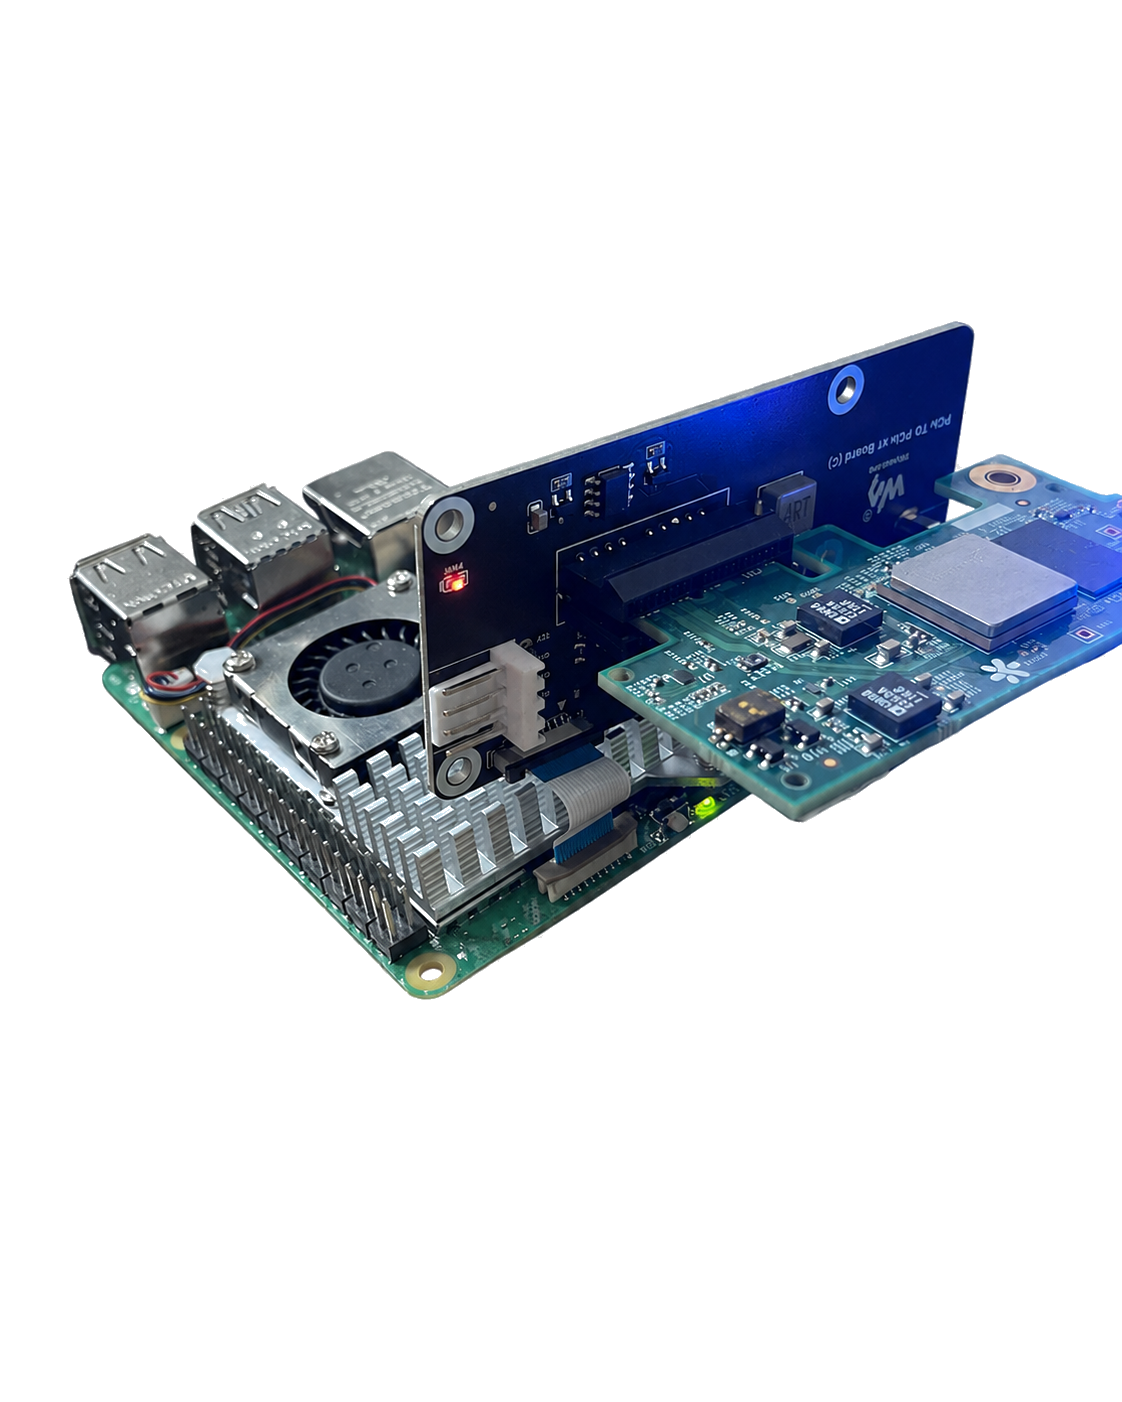
\includegraphics[width=0.60\textwidth]{hardware-powered-isolated.png}
  \vfill
  {\large Álvaro Poveda Ruiz\par}
  \vspace{2mm}
  {\small Manual de usuario\par
  Universidad Politécnica de Madrid, 2026\par}
  \vspace{8mm}
  {\small Versión \versionmanual{} · Revisión: \fechacorte\par}
\end{titlepage}

\chapter*{Resumen}
\addcontentsline{toc}{chapter}{Resumen}

Este manual describe la puesta en marcha de una tarjeta BrainChip AKD1000 conectada por PCIe.
El procedimiento incluye la preparación del equipo, la instalación del controlador y del
entorno de Python, la carga de un modelo y la comprobación de su ejecución. También explica
cómo medir la latencia y localizar los fallos más habituales.

La primera prueba utiliza un modelo sencillo cuya salida se conoce de antemano. Se ejecuta
primero en software y después en la tarjeta. Así se puede comprobar por separado el
funcionamiento del entorno de Akida, la compatibilidad del modelo y el acceso al hardware
antes de utilizar una aplicación propia.

La ejecución completa de esta versión del procedimiento en una placa física sigue pendiente.

\section*{Alcance del manual}

El manual cubre las operaciones necesarias para instalar el entorno, detectar la tarjeta,
cargar y ejecutar modelos, consultar las estadísticas y medir el rendimiento.
También incluye comprobaciones para localizar errores de conexión, controlador, datos o modelo.

Las instrucciones de montaje deben aplicarse a la revisión concreta de cada componente.
Antes de conectar la alimentación, hay que comprobar la tensión, la polaridad y la orientación
del cable en la documentación del fabricante. El manual no cubre la reparación electrónica
de la tarjeta ni su diseño interno.

\chapter*{Cómo usar este documento}
\addcontentsline{toc}{chapter}{Cómo usar este documento}

Descarga el PDF junto con \code{akd1000-bringup.zip} y extrae el ZIP. Abre una terminal
en la carpeta \projectroot, donde están \code{pyproject.toml}, \code{examples/} y
\code{models/}. Todos los comandos del proyecto parten de esa carpeta, salvo que se indique otra.
No ejecutes los ejemplos desde el visor del ZIP. Conserva el PDF y el ZIP con la misma versión.

Ejecuta solo el bloque que corresponda a tu equipo.
Los bloques que usan \code{sudo}, \code{apt} o \code{lspci} son para Linux. El
\cref{chap:software} incluye la activación del entorno en Windows.

Si trabajas sin tarjeta, empieza por el \cref{chap:software} y completa la prueba en software.
Si dispones del hardware, lee primero el inventario y el montaje de los capítulos
\ref{chap:orientacion} y \ref{chap:hardware}; después prepara el controlador y el SDK.

\section*{Versión y material incluido}

\begin{tabularx}{\textwidth}{@{}L{0.29\textwidth}Y@{}}
\toprule
\textbf{Campo} & \textbf{Valor} \\
\midrule
Versión y fecha & \versionmanual{}; \fechacorte \\
Fuente editable & \code{manual/main.tex} y \code{manual/sections/} \\
Pruebas de esta edición & Pruebas automatizadas y simulador con Akida 2.19.1 y 2.19.3 en Windows; ejecución física pendiente \\
Modelo incluido & \code{models/akida\_v1\_smoke\_test.fbz}; cuatro entradas y dos salidas \\
\bottomrule
\end{tabularx}

Las referencias finales contienen enlaces a las instrucciones oficiales. La ruta de software
actual y la compatibilidad del controlador se comprueban por separado: que un SDK se instale
no garantiza que el kernel pueda cargar el controlador PCIe.

\tableofcontents
\clearpage
\begingroup
\let\clearpage\relax
\let\cleardoublepage\relax
\listoffigures
\listoftables
\endgroup

\chapter{Orientación y elección de ruta}
\label{chap:orientacion}

\section{Qué componentes intervienen}

La AKD1000 no se maneja como una aplicación aislada. El host ejecuta el sistema operativo y el
runtime; PCIe transporta órdenes y datos; el controlador expone el dispositivo al sistema; y el
modelo FBZ define la red que el runtime puede mapear. Separar estas capas evita buscar un fallo
de alimentación en Python o intentar resolver un paquete ausente reinstalando el controlador.

\begin{table}[H]
\centering
\caption{Responsabilidad de cada capa del sistema.}
\label{tab:capas}
\begin{tabularx}{\textwidth}{@{}L{0.22\textwidth}YY@{}}
\toprule
\textbf{Capa} & \textbf{Qué hace} & \textbf{Qué no demuestra por sí sola} \\
\midrule
Host & Ejecuta Linux o Windows, Python, preparación de datos y registros. & Que el cálculo se haya realizado en la tarjeta. \\
Interfaz PCIe & Transporta configuración, entradas y salidas. & Que exista un controlador utilizable. \\
Controlador Linux & Crea el acceso al dispositivo, normalmente mediante \code{/dev/akida*}. & Que el modelo sea compatible. \\
Runtime Akida & Carga FBZ, descubre dispositivos, mapea y ejecuta. & Que un mapeo virtual sea una inferencia física. \\
AKD1000 & Ejecuta las secuencias asignadas al hardware. & El tiempo total de Python ni el consumo de toda la plataforma. \\
FBZ & Conserva una red Akida serializada. & El significado de las entradas, las etiquetas o el dataset. \\
\bottomrule
\end{tabularx}
\end{table}

La tarjeta PCIe documentada por BrainChip contiene un AKD1000, usa una interfaz host PCIe y
dispone de memoria LPDDR4 accesible mediante DMA \cite{brainchip_card_brief}. El product brief
del SoC describe veinte núcleos de procesamiento neuronal y un endpoint PCIe 2.1 de dos líneas
\cite{brainchip_soc_brief}. Estas son características del producto; no son una promesa de
latencia, energía o utilización para cualquier red.

\section{Tres decisiones antes de empezar}

\paragraph{Decisión 1: software o hardware.}
Si aún no tienes una tarjeta, sigue la ruta \textbf{S}: entorno software, modelo de prueba y
dispositivo virtual. Si tienes la tarjeta y una conexión PCIe documentada, completa primero la
ruta S y continúa con la ruta \textbf{H}. La simulación confirma el modelo y el paquete; no
confirma el cableado, el controlador ni la placa.


\paragraph{Decisión 2: entorno actual o de referencia.}
Para aprender con la documentación vigente usa la ruta \textbf{A}: MetaTF 2.19.3, o la versión
que figure en la página oficial cuando leas el manual. Para repetir la prueba incluida usa la ruta
\textbf{R}: Python 3.11 y Akida 2.19.1.
No mezcles ambas instalaciones
en el mismo entorno virtual.


\paragraph{Decisión 3: tipo de host.}
Un PC Linux con ranura PCIe y una Raspberry Pi 5 con adaptador FFC requieren montajes distintos.
Windows está incluido en las configuraciones software actuales de MetaTF
\cite{brainchip_install_2193}, pero este manual no afirma soporte de la tarjeta física en
Windows: las instrucciones del controlador PCIe público consultado son para Linux
\cite{brainchip_driver}.


\section{Matriz de rutas}

\begin{longtable}{@{}L{0.12\textwidth}L{0.21\textwidth}L{0.29\textwidth}L{0.28\textwidth}@{}}
\caption{Recorridos cubiertos por el manual.}\label{tab:rutas}\\
\toprule
\textbf{Ruta} & \textbf{Equipo} & \textbf{Objetivo} & \textbf{Evidencia final} \\
\midrule
\endfirsthead
\toprule
\textbf{Ruta} & \textbf{Equipo} & \textbf{Objetivo} & \textbf{Evidencia final} \\
\midrule
\endhead
S & Windows o Linux compatible, sin tarjeta & Instalar MetaTF, importar Akida y ejecutar en software. & Versión registrada, salida del modelo y mapeo virtual. \\
H-PC & Host Linux, tarjeta y conexión PCIe documentada & Detectar y ejecutar en AKD1000 mediante el controlador público. & \code{lspci}, módulo, nodo, \code{akida devices} y prueba física. \\
H-Pi & Raspberry Pi 5, adaptador FFC y tarjeta & Habilitar PCIe cuando proceda y completar H-PC. & Configuración de arranque, enumeración y prueba física. \\
R & Python 3.11 y SDK de referencia & Repetir la prueba básica con Akida 2.19.1. & Salida conocida y mapeo virtual comprobado. \\
\bottomrule
\end{longtable}

\section{Comprobar cada etapa}

Cada etapa responde a una pregunta distinta:

\begin{enumerate}[nosep]
  \item \textbf{Inventario:} ¿sé exactamente qué host, tarjeta, adaptador, fuentes, sistema,
        kernel y arquitectura tengo?
  \item \textbf{Montaje:} ¿la cadena está conectada según la documentación de esas revisiones?
  \item \textbf{Enumeración:} ¿el host ve un endpoint PCIe nuevo?
  \item \textbf{Controlador:} ¿el módulo se ha compilado para este kernel y existe acceso al nodo?
  \item \textbf{SDK:} ¿el intérprete activo importa la versión prevista de Akida?
  \item \textbf{Modelo:} ¿el FBZ carga, tiene el contrato esperado y mapea como se pretende?
  \item \textbf{Ejecución:} ¿una entrada conocida produce una salida conocida en hardware?
  \item \textbf{Medida:} ¿la ventana, las unidades y la frontera de potencia están declaradas?
\end{enumerate}

Resuelve la primera etapa que falla antes de continuar. Guarda su error para localizar
el problema.

\chapter{Hardware, alimentación y montaje}
\label{chap:hardware}

\section{Inventario del montaje}

Antes de empezar, anota los datos que puedas comprobar de cada componente.
No completes una referencia a partir de una fotografía o por parecido con otro modelo.
Si algún dato, como la revisión de una placa o su tensión de alimentación, no puede
confirmarse con la etiqueta, la factura o la documentación del fabricante, indícalo como
\emph{no verificado}.

\begin{table}[H]
\centering
\caption{Datos básicos del montaje.}
\label{tab:inventario-lector}
\begin{tabularx}{\textwidth}{@{}L{0.28\textwidth}L{0.31\textwidth}Y@{}}
\toprule
\textbf{Elemento} & \textbf{Datos} & \textbf{Fuente} \\
\midrule
Host & Fabricante, modelo, RAM y revisión & Equipo, firmware o factura \\
Sistema & Distribución, versión y arquitectura & \code{/etc/os-release}, \code{uname -m} \\
Kernel & Versión completa & \code{uname -r} \\
Tarjeta Akida & Modelo y revisión & Etiqueta y documentación de BrainChip \\
Adaptador & Fabricante, modelo y tipo de enlace & Serigrafía y documentación del fabricante \\
Cable & Tipo y orientación & Marcado y documentación del adaptador \\
Fuente del host & Tensión y potencia & Etiqueta de la fuente \\
Fuente de la tarjeta o carrier & Tensión, polaridad y conector & Etiqueta y documentación del fabricante \\
\bottomrule
\end{tabularx}
\end{table}

Los conectores M.2, Mini PCIe, PCIe convencional y el conector FFC de Raspberry Pi 5
no son equivalentes. Comprueba siempre el tipo de conexión y la orientación del cable
en la documentación del equipo utilizado.

\section{Topologías cubiertas}

\subsection{Host Linux con ranura PCIe}

En un PC Linux, la tarjeta se instala en una ranura PCIe compatible y se alimenta según
las indicaciones de su documentación. El equipo debe estar apagado y desconectado antes
de insertar o retirar la tarjeta.

Después del montaje, continúa con el \cref{chap:host-driver}. Si \code{lspci}
no detecta un nuevo dispositivo PCIe, el problema debe resolverse antes de continuar
con la configuración de Python.

\subsection{Raspberry Pi 5 con adaptador FFC a PCIe}

Raspberry Pi 5 dispone de una interfaz PCIe Gen~2~$\times$1 accesible mediante un
conector FFC \cite{rpi_pcie}. Para utilizar una tarjeta PCIe convencional es necesario
un adaptador que lleve este enlace hasta una ranura compatible.

Aunque el adaptador disponga de una ranura físicamente más larga, el enlace proporcionado
por Raspberry Pi 5 sigue siendo $\times$1.

El montaje del TFG se muestra en la \cref{fig:montaje-aislado}.

\begin{figure}[H]
  \centering
  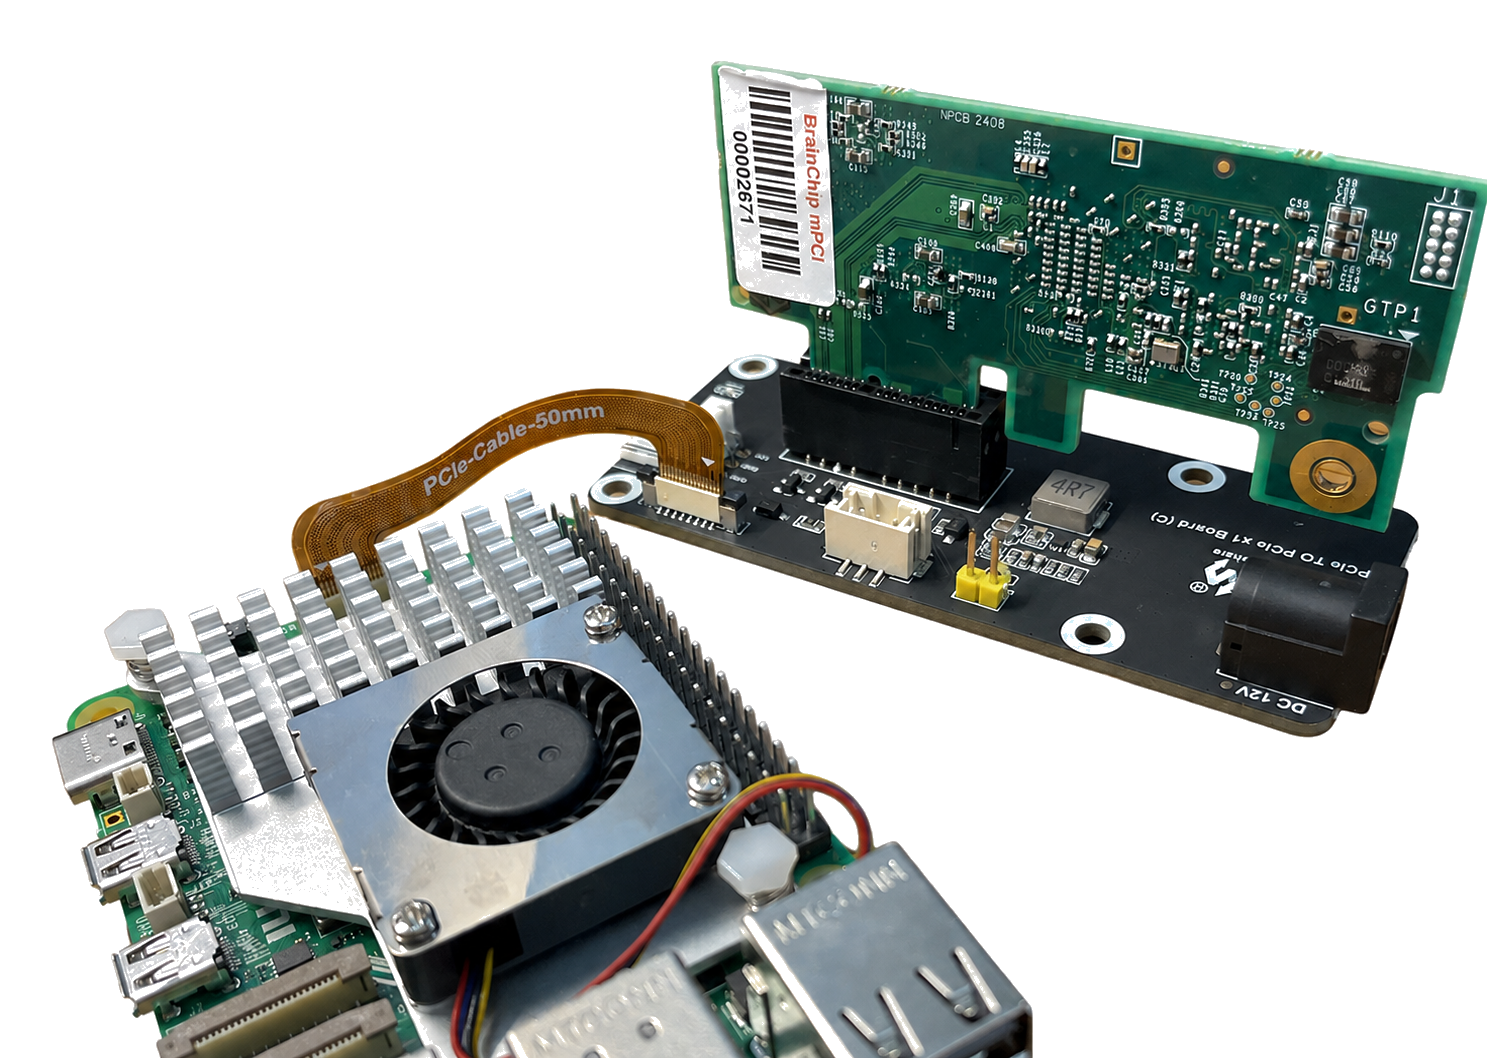
\includegraphics[width=0.92\textwidth]{hardware-carrier-detail-isolated.png}
  \caption[Montaje Raspberry Pi 5, carrier y AKD1000]{Montaje formado por una Raspberry Pi 5,
  un adaptador PCIe y la tarjeta BrainChip AKD1000 utilizado durante el TFG.}
  \label{fig:montaje-aislado}
\end{figure}

\section{Montaje}

Si la documentación del fabricante indica una secuencia de conexión diferente,
sigue ese procedimiento.

\begin{enumerate}
  \item Apaga el host y desconecta las fuentes de alimentación.

  \item Comprueba la orientación del cable FFC y la tensión de alimentación del
        adaptador o de la tarjeta.

  \item Conecta el cable FFC al adaptador respetando la orientación indicada.

  \item Inserta la AKD1000 completamente en la ranura PCIe del carrier.

  \item Revisa las conexiones antes de alimentar de nuevo el sistema.
\end{enumerate}

\begin{stopbox}{Si aparece algún problema eléctrico}
Desconecta la alimentación si aparece humo, olor anormal, una temperatura excesiva
o cualquier otro comportamiento que indique un posible problema de alimentación
o montaje.
\end{stopbox}

\section{Carrier Waveshare utilizado en el TFG}

En el montaje del TFG se utilizó un adaptador Waveshare conectado a la Raspberry Pi 5
mediante un cable FFC de 50~mm. En la placa puede leerse \code{DC 12V} y
\emph{PCIe TO PCIe x1 Board (C)}.

La documentación actual de Waveshare describe este modelo con una ranura compatible
mecánicamente con tarjetas PCIe $\times$1, $\times$4, $\times$8 y $\times$16
\cite{waveshare_board_c}. El enlace con Raspberry Pi 5 continúa siendo, en cualquier caso,
PCIe $\times$1.

No se conserva el número de artículo exacto del adaptador utilizado. La identificación
disponible del montaje se recoge en el \cref{tab:componentes-tfg}.

\begin{figure}[H]
  \centering
  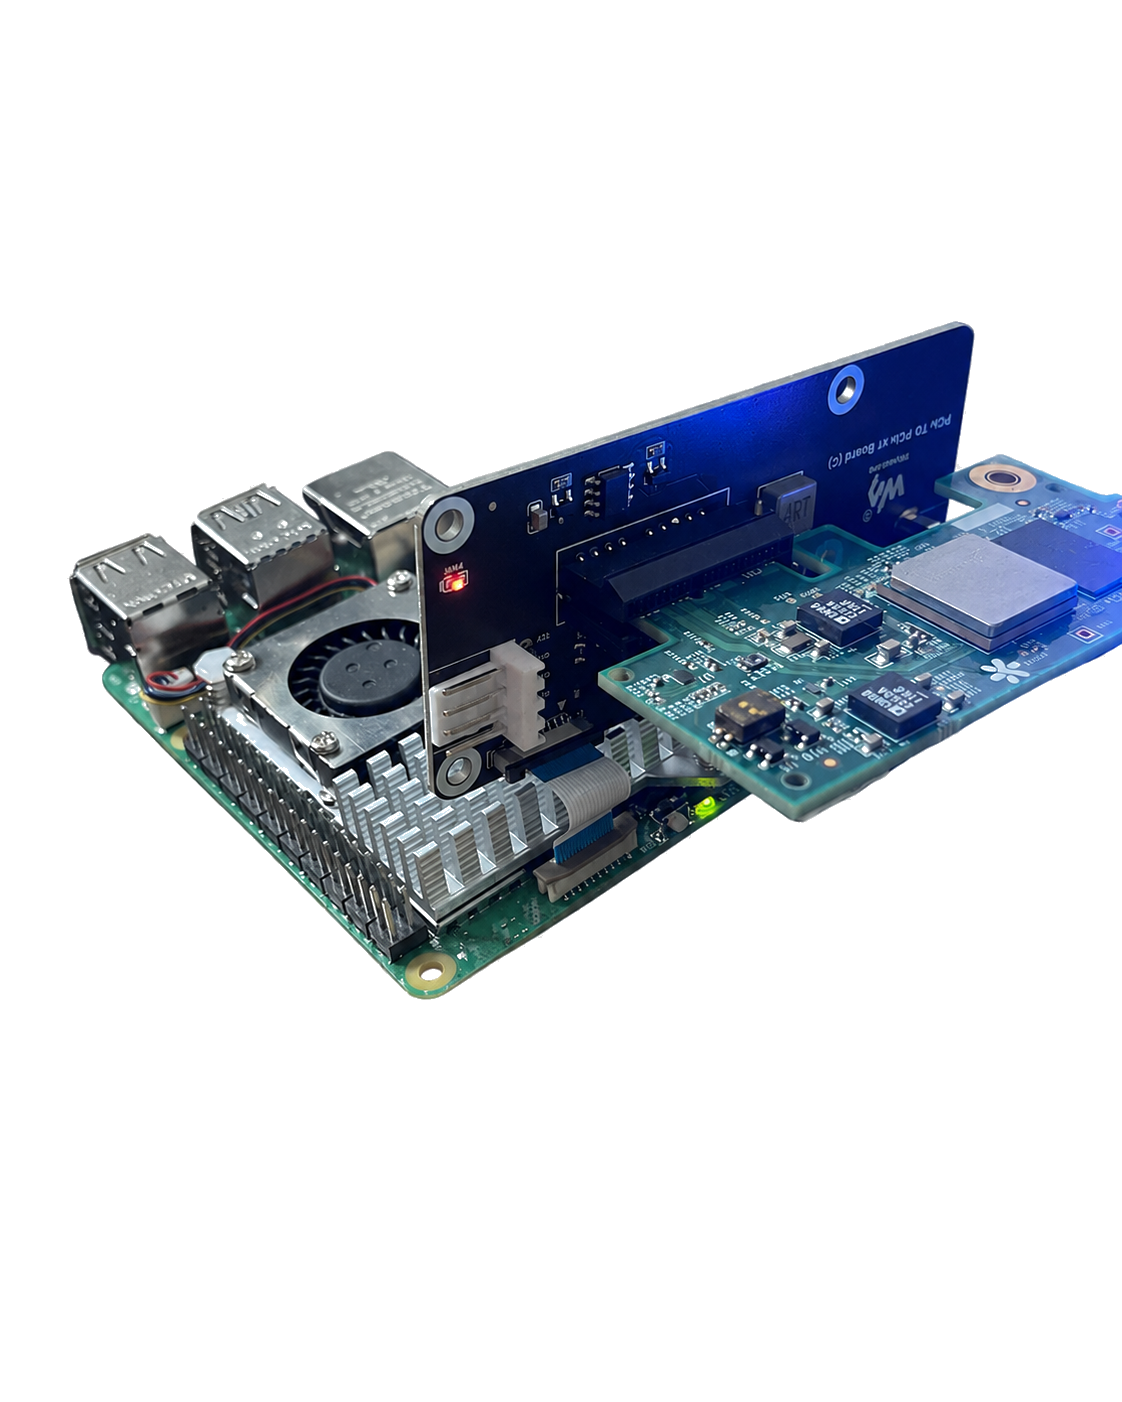
\includegraphics[width=0.78\textwidth]{hardware-powered-isolated.png}
  \caption[Montaje alimentado]{Montaje utilizado durante una de las sesiones del TFG.}
  \label{fig:montaje-alimentado}
\end{figure}

\section{Comprobación antes del encendido}

Antes de alimentar el montaje, comprueba que el cable FFC está correctamente orientado,
que la tarjeta está bien insertada y que las tensiones de alimentación coinciden con las
indicadas para los componentes utilizados.

\begin{stopbox}{Condición de parada H0}
Si no puedes confirmar la tensión, la polaridad o la orientación de alguna conexión,
no alimentes el montaje hasta comprobarlo en la documentación correspondiente.
\end{stopbox}
\chapter{Preparación del host y controlador PCIe}
\label{chap:host-driver}

\section{Comprobaciones iniciales}

Antes de instalar el controlador, comprueba la versión del sistema, la arquitectura y el kernel.
En Linux puedes guardar esta información en la carpeta \code{evidence}:

\begin{lstlisting}[language=bash]
mkdir -p evidence
{
  cat /etc/os-release
  uname -r
  uname -m
  lspci -nn
} | tee evidence/host-inventory.txt
\end{lstlisting}

\code{uname -m} suele mostrar \code{x86\_64} en un PC y \code{aarch64} en una
Raspberry Pi 5 con un sistema de 64 bits. La versión del kernel será necesaria para
comprobar la compatibilidad del controlador.

\section{Habilitar PCIe en Raspberry Pi 5}

Esta sección solo es necesaria si utilizas una Raspberry Pi 5. Los dispositivos HAT+
compatibles pueden detectarse automáticamente, mientras que para un adaptador PCIe no HAT+
Raspberry Pi indica que debe habilitarse la interfaz PCIe en el archivo de configuración
\cite{rpi_pcie}.

En Raspberry Pi OS actual, abre:

\begin{lstlisting}[language=bash]
sudoedit /boot/firmware/config.txt
\end{lstlisting}

Si esa ruta no existe, comprueba \code{/boot/config.txt}. Añade:

\begin{lstlisting}[language=bash]
dtparam=pciex1
\end{lstlisting}

Guarda el archivo y reinicia:

\begin{lstlisting}[language=bash]
sudo reboot
\end{lstlisting}

Raspberry Pi 5 utiliza PCIe Gen2 por defecto. Aunque es posible habilitar Gen3,
Raspberry Pi advierte que la placa no está certificada para funcionar de forma estable
a esa velocidad \cite{rpi_pcie}. Para la puesta en marcha se mantiene Gen2.

\section{Comprobar la conexión PCIe}

Después del arranque, comprueba que el sistema detecta la tarjeta:

\begin{lstlisting}[language=bash]
lspci -nn
\end{lstlisting}

Debe aparecer un dispositivo PCIe correspondiente a la tarjeta. Si no aparece, revisa
el montaje, la alimentación y, en Raspberry Pi 5, que PCIe esté habilitado antes de
continuar con el controlador.

Si necesitas más información sobre el dispositivo detectado, utiliza:

\begin{lstlisting}[language=bash]
lspci -nnk
\end{lstlisting}

En este punto solo se está comprobando la conexión PCIe. Que la tarjeta aparezca en
\code{lspci} no significa todavía que el controlador Akida esté instalado.

\section{Instalar el controlador}

El controlador PCIe oficial de BrainChip se distribuye en el repositorio
\code{akida\_dw\_edma}. Antes de instalarlo, comprueba la versión del kernel:

\begin{lstlisting}[language=bash]
uname -r
\end{lstlisting}

La versión del controlador consultada para este manual admite kernels desde 5.4 hasta
6.8. En kernels 6.9 o posteriores el módulo no se compila \cite{brainchip_driver}.
Como esta compatibilidad puede cambiar, consulta también el README del
repositorio antes de instalarlo.

\paragraph{Kernel no compatible.}
Si la versión del kernel queda fuera del intervalo soportado por el controlador,
no continúes con la instalación hasta comprobar si BrainChip ha publicado una versión
compatible.


En Ubuntu, instala las dependencias indicadas por BrainChip:

\begin{lstlisting}[language=bash]
sudo apt update
sudo apt install dkms build-essential "linux-headers-$(uname -r)"
\end{lstlisting}

En otras distribuciones los nombres de los paquetes pueden cambiar, pero deben
instalarse DKMS, las herramientas de compilación y los headers correspondientes al
kernel en uso.

A continuación, clona el repositorio e instala el controlador:

\begin{lstlisting}[language=bash]
git clone https://github.com/Brainchip-Inc/akida_dw_edma.git
cd akida_dw_edma
git rev-parse HEAD
./install.sh
\end{lstlisting}

La salida de \code{git rev-parse HEAD} registra la revisión exacta del controlador
utilizada; también puedes usar una configuración propia.

\section{Comprobar el controlador}

Después de instalar el controlador, revisa el estado de DKMS y confirma que el dispositivo
Akida está disponible:

\begin{lstlisting}[language=bash]
dkms status
lsmod | grep -i akida
ls -l /dev/akida*
lspci -nnk
\end{lstlisting}

La instalación puede considerarse correcta cuando el dispositivo sigue apareciendo
en PCIe, el módulo está cargado y existe al menos un nodo \code{/dev/akida*}.

Si el dispositivo aparece en \code{lspci} pero falta \code{/dev/akida*}, consulta los
mensajes del kernel:

\begin{lstlisting}[language=bash]
sudo dmesg | grep -iE 'akida|edma|pcie' | tail -n 120
\end{lstlisting}

Si el nodo existe pero solo puede utilizarse como \code{root}, revisa sus permisos y
la regla udev instalada por el controlador antes de continuar.

Con el controlador funcionando, continúa con la configuración del entorno de software
del \cref{chap:software}.

\chapter{Entorno de software y primera prueba}
\label{chap:software}

\section{Preparar el entorno}

BrainChip distribuye las herramientas de Akida mediante MetaTF. En la versión utilizada
para este manual, la instalación actual emplea \code{metatf==2.19.3} y admite
Python 3.10--3.12 \cite{brainchip_install_2193}.

El repositorio también incluye una configuración de referencia basada en Python 3.11
y Akida 2.19.1, la misma versión utilizada durante el TFG. Esta segunda opción permite
repetir la prueba básica con un entorno conocido.

Abre una terminal en \projectroot, la carpeta extraída del ZIP.

En Linux:

\begin{lstlisting}[language=bash]
python3.11 -m venv .venv
source .venv/bin/activate
python -m pip install --upgrade pip
\end{lstlisting}

En Windows, PowerShell:

\begin{lstlisting}
py -3.11 -m venv .venv
.\.venv\Scripts\Activate.ps1
python -m pip install --upgrade pip
\end{lstlisting}

El entorno virtual solo se crea una vez. En una terminal nueva basta con volver a
activarlo antes de continuar.

\section{Instalar Akida}

Elige una de las dos configuraciones siguientes.

Para trabajar con la versión actual documentada por BrainChip:

\begin{lstlisting}
python -m pip install "metatf==2.19.3"
\end{lstlisting}

Para repetir la configuración de referencia incluida con el repositorio:

\begin{lstlisting}
python -m pip install -r requirements/reproducible.txt
\end{lstlisting}

No mezcles ambas instalaciones en el mismo entorno virtual.

A continuación, instala las herramientas incluidas con este repositorio:

\begin{lstlisting}
python -m pip install -e . --no-deps
python -m pip check
\end{lstlisting}

Comprueba que Akida se importa correctamente:

\begin{lstlisting}
python -c "import akida; print(akida.__version__); print(akida.devices())"
\end{lstlisting}

Si no hay una tarjeta conectada, es normal que \code{akida.devices()} devuelva
\code{[]}. Si el equipo tiene una AKD1000 conectada y el controlador está funcionando,
debe aparecer al menos un dispositivo.

\section{Primera prueba en software}

Antes de utilizar la tarjeta, ejecuta el modelo de prueba incluido con el repositorio:

\begin{lstlisting}
python examples/00_simulator_smoke.py
\end{lstlisting}

El modelo recibe cuatro valores de entrada. Para

\begin{lstlisting}
[3, 2, 1, 4]
\end{lstlisting}

la salida esperada es

\begin{lstlisting}
[5, 5]
\end{lstlisting}

El script ejecuta primero el modelo en software y comprueba después que puede mapearse
sobre un AKD1000 virtual. Este último paso verifica la compatibilidad del modelo con la
arquitectura de la tarjeta, pero no utiliza hardware físico.

También puedes ejecutar la comprobación incluida en la herramienta del repositorio:

\begin{lstlisting}
akd1000-bringup verify --id smoke --model models/akida_v1_smoke_test.fbz
\end{lstlisting}

Si ambas pruebas terminan correctamente, el entorno de Python y el modelo de prueba
están preparados.

\section{Comprobar el equipo}

Antes de usar la tarjeta física, puedes ejecutar el diagnóstico incluido con el
repositorio:

\begin{lstlisting}
akd1000-bringup doctor
\end{lstlisting}

Para guardar el resultado:

\begin{lstlisting}
mkdir -p evidence
akd1000-bringup doctor --json > evidence/preflight.json
\end{lstlisting}

La herramienta comprueba, entre otros datos, la versión de Akida, el kernel, la conexión
PCIe y los dispositivos detectados. Su salida ayuda a localizar el problema si la tarjeta no aparece.

En un equipo sin AKD1000 es normal que el diagnóstico indique que no se ha encontrado
ningún dispositivo.

\section{Primera ejecución en la AKD1000}

Esta prueba requiere que la tarjeta haya sido detectada por PCIe y que el controlador
del \cref{chap:host-driver} esté instalado.

Comprueba primero que Akida detecta el dispositivo:

\begin{lstlisting}
akida devices
\end{lstlisting}

Después ejecuta:

\begin{lstlisting}
python examples/01_hardware_smoke.py
\end{lstlisting}

El script carga el mismo modelo utilizado en la prueba de software, lo mapea sobre la
AKD1000 y ejecuta la entrada conocida. La salida debe volver a ser:

\begin{lstlisting}
[5, 5]
\end{lstlisting}

Un resultado \code{PASS} confirma que el modelo se ha cargado, que la tarjeta es
accesible desde Akida y que la inferencia se ha ejecutado correctamente en el hardware.

\paragraph{Si la prueba física falla.}
No continúes todavía con un modelo propio. Conserva el mensaje de error y utiliza el
procedimiento de diagnóstico del \cref{chap:diagnostico} para localizar el problema.

\chapter{Operación de modelos Akida}
\label{chap:operacion}

\section{Cargar e inspeccionar un modelo}

Los modelos Akida se distribuyen como archivos FBZ. Antes de ejecutarlos conviene conocer,
al menos, la forma de entrada, la forma de salida y el preprocesado utilizado durante su
conversión.

Carga el modelo y revisa su estructura:

\begin{lstlisting}[language=Python]
import akida

model = akida.Model("models/model.fbz")

print("input_shape:", model.input_shape)
print("output_shape:", model.output_shape)
print("ip_version:", model.ip_version)
model.summary()
\end{lstlisting}

\code{summary()} muestra las capas y la forma en la que el modelo puede ejecutarse.
La cantidad de recursos utilizados depende del propio modelo y del modo de mapeo.

\section{Seleccionar el dispositivo}

Los dispositivos físicos disponibles se obtienen mediante \code{akida.devices()}
\cite{brainchip_akida_guide}:

\begin{lstlisting}[language=Python]
import akida

devices = list(akida.devices())

if not devices:
    raise RuntimeError("No se ha detectado ningun dispositivo Akida")

device = devices[0]
print(device)
\end{lstlisting}

Un dispositivo creado con \code{akida.AKD1000()} es virtual y sirve para comprobar
el mapeo de un modelo. Para ejecutar una inferencia en la tarjeta es necesario utilizar
uno de los dispositivos devueltos por \code{akida.devices()}.

\section{Mapear el modelo en la tarjeta}

Un modelo cargado puede ejecutarse inicialmente mediante software. Para utilizar la AKD1000
debe mapearse sobre el dispositivo:

\begin{lstlisting}[language=Python]
model.map(
    device,
    hw_only=True,
    mode=akida.MapMode.AllNps
)

model.summary()
\end{lstlisting}

Con \code{hw\_only=True} se exige que la ejecución se realice completamente en el hardware
Akida \cite{brainchip_akida_guide}. Si el modelo no puede mapearse de esta forma, la llamada
produce un error.

\code{AllNps}, \code{HwPr} y \code{Minimal} son distintos modos de asignar los recursos
de la AKD1000. Para una primera ejecución puedes usar \code{AllNps}. Su efecto sobre
latencia y consumo se estudia en el \cref{chap:rendimiento}.

\section{Preparar la entrada}

La forma y el tipo de los datos dependen del modelo. Antes de ejecutar una inferencia,
comprueba que la entrada coincide con \code{model.input\_shape}.

Por ejemplo, para datos almacenados en NumPy:

\begin{lstlisting}[language=Python]
import numpy as np

data = np.load("data/inputs.npy", allow_pickle=False)

print("shape:", data.shape)
print("dtype:", data.dtype)
print("min/max:", data.min(), data.max())

if tuple(data.shape[1:]) != tuple(model.input_shape):
    raise ValueError(
        f"Forma de entrada {data.shape[1:]} "
        f"!= {model.input_shape}"
    )
\end{lstlisting}

El tipo, el rango y el orden de los canales deben ser los mismos utilizados durante
la preparación y conversión del modelo. No existe un rango de entrada común para todos
los modelos Akida.


\section{Ejecutar el modelo}

La API de Akida permite ejecutar el modelo mediante \code{forward()} o \code{predict()}.
La elección depende de cómo se haya definido la salida del modelo y de cómo se haya
validado durante su conversión \cite{brainchip_akida_guide}.

Por ejemplo:

\begin{lstlisting}[language=Python]
output = model.forward(data)
print(output)
\end{lstlisting}

Durante una campaña de medidas debe mantenerse el mismo método de ejecución para que
los resultados sean comparables.

También puedes usar la herramienta incluida en este repositorio:

\begin{lstlisting}[language=bash]
akd1000-bringup run \
  --model models/model.fbz \
  --input data/input.npy \
  --method forward \
  --clock Performance \
  --map AllNps \
  --output outputs/raw-output.npy
\end{lstlisting}

La herramienta carga la entrada, ejecuta el modelo y guarda la salida en un archivo NumPy.
La entrada debe tener la forma

\begin{lstlisting}
(batch, *model.input_shape)
\end{lstlisting}

Los modelos con varias entradas o salidas requieren tratarlos directamente mediante
la API de Akida.

\section{Modo de reloj}

La AKD1000 dispone de los modos de reloj \code{Performance}, \code{Economy} y
\code{LowPower}. El modo puede seleccionarse mediante la API:

\begin{lstlisting}[language=Python]
device.soc.clock_mode = akida.soc.ClockMode.Performance
print(device.soc.clock_mode)
\end{lstlisting}

El modo de reloj debe anotarse cuando se comparen medidas de rendimiento. Un modo de menor
potencia instantánea no implica necesariamente una menor energía por inferencia, ya que también
puede cambiar el tiempo de ejecución.
\chapter{Medida de rendimiento y energía}
\label{chap:medida}
\label{chap:rendimiento}

\section{Qué se está midiendo}

Antes de comparar resultados, mantén fijos el modelo, los datos y la configuración de
ejecución. Anota también el modo de reloj, el modo de mapeo y el número de repeticiones.


\section{Medida de latencia}

La herramienta mide el tiempo empleado por la llamada de ejecución del modelo. La medida
incluye la comunicación entre el host y la tarjeta, la llamada al SDK y la inferencia en
la AKD1000.

La carga de los archivos, el mapeo del modelo y las ejecuciones de calentamiento se realizan
antes de comenzar a medir.

\begin{figure}[H]
  \centering
  \begin{tikzpicture}[
    stage/.style={draw=black!70,align=center,
                  minimum height=12mm,text width=25mm,fill=white},
    flow/.style={->,thick,draw=black}
  ]
    \node[stage] (input) at (-4.8,0) {Entrada};
    \node[stage] (host) at (-1.6,0) {Host\\API Akida};
    \node[stage] (device) at (1.6,0) {AKD1000\\inferencia};
    \node[stage] (output) at (4.8,0) {Salida};

    \draw[flow] (input) -- (host);
    \draw[flow] (host) -- (device);
    \draw[flow] (device) -- (output);

    \draw[dashed,black!70]
      (-1.6,0.9) -- (-1.6,1.2) -- (4.8,1.2) -- (4.8,0.9);

    \node[fill=white,inner sep=1mm] at (1.6,1.2)
      {Latencia observada desde el host};
  \end{tikzpicture}

  \caption[Frontera de la medida de latencia]
  {Elementos incluidos en la medida de latencia realizada desde el host.}
  \label{fig:measurement-boundary}
\end{figure}

Por tanto, los resultados de este manual se expresan como
\emph{latencia observada desde el host}. No corresponden a un temporizador interno aislado
del AKD1000.

Si se quiere medir el tiempo completo de una aplicación, deben añadirse también las etapas
de adquisición, preprocesado y postprocesado.

\section{Ejecutar un benchmark}

Antes de una campaña completa, ejecuta una prueba corta para comprobar que el
modelo, los datos y la configuración son correctos.

\begin{lstlisting}[language=bash]
akd1000-bringup benchmark \
  --model models/model.fbz \
  --input data/inputs.npy \
  --method forward \
  --clock Performance \
  --map AllNps \
  --warmup 8 \
  --repetitions 1 \
  --output outputs/smoke
\end{lstlisting}

La carpeta de salida contiene:

\begin{itemize}
  \item \code{latencies.csv}, con las medidas individuales;
  \item \code{summary.json}, con la configuración y el resumen del ensayo;
  \item \code{host.json}, con información del sistema utilizado.
\end{itemize}

Comprueba que el número de muestras, las unidades y la configuración son los esperados.
Si la prueba es correcta, repite el benchmark con el número de repeticiones necesario y
guarda los resultados en una carpeta distinta.

Para comparar configuraciones, cambia una sola variable cada vez. Por ejemplo, puedes
mantener fijo el modelo y comparar los modos \code{AllNps}, \code{HwPr} y \code{Minimal},
o mantener fijo el mapeo y cambiar el modo de reloj.

\section{Potencia y energía}

Akida permite habilitar la medida de potencia del dispositivo y consultar las estadísticas
después de una inferencia \cite{brainchip_akida_guide}:

\begin{lstlisting}[language=Python]
device.soc.power_measurement_enabled = True

model.forward(data)

print(model.statistics)
\end{lstlisting}

La potencia proporcionada por esta API corresponde a la medida disponible en el dispositivo.
No representa el consumo completo de la Raspberry Pi, el carrier y la tarjeta.

Con una potencia media y la latencia medida desde el host, puede calcularse
una energía estimada por inferencia como

\begin{equation}
  E_{\mathrm{est}} \,[\mu\mathrm{J}]
  =
  P_{\mathrm{API}} \,[\mathrm{mW}]
  \,
  t_{\mathrm{host}} \,[\mathrm{ms}].
\end{equation}

La relación de unidades es directa:

\[
1\,\mathrm{mW}\cdot 1\,\mathrm{ms}
=
1\,\mu\mathrm{J}.
\]

Esta estimación combina la potencia de la API con la latencia observada desde el host.
Permite comparar ejecuciones con el mismo procedimiento; no mide la energía interna
del chip ni el consumo energético total del sistema.

Para medir el consumo completo sería necesario utilizar instrumentación externa sobre la
alimentación del montaje.

\section{Guardar los resultados}

Para cada ensayo conserva, como mínimo:

\begin{itemize}
  \item el modelo y su versión;
  \item los datos utilizados;
  \item el modo de reloj;
  \item el modo de mapeo;
  \item el número de repeticiones;
  \item los archivos generados por el benchmark.
\end{itemize}

Si se comparan distintas plataformas, como CPU, GPU o FPGA, deben utilizarse la misma tarea,
los mismos datos y una definición equivalente de la medida.

\chapter{Diagnóstico}
\label{chap:diagnostico}

Cuando aparece un error, conviene comprobar el sistema en el mismo orden seguido durante
la puesta en marcha: conexión PCIe, controlador, entorno de Python, modelo y datos.
La \cref{tab:troubleshooting} resume los fallos más habituales y dónde empezar a buscarlos.

\begin{longtable}{@{}L{0.25\textwidth}L{0.34\textwidth}L{0.33\textwidth}@{}}
\caption{Guía rápida de diagnóstico.}
\label{tab:troubleshooting}\\
\toprule
\textbf{Síntoma} & \textbf{Comprueba} & \textbf{Qué hacer} \\
\midrule
\endfirsthead

\toprule
\textbf{Síntoma} & \textbf{Comprueba} & \textbf{Qué hacer} \\
\midrule
\endhead

La tarjeta no aparece en \code{lspci}. &
Alimentación, cable FFC, montaje y configuración PCIe de la Raspberry Pi 5. &
Revisa primero la conexión física y la configuración PCIe. \\

La tarjeta aparece en PCIe, pero no existe \code{/dev/akida*}. &
Versión del kernel, headers, \code{dkms status}, \code{lsmod} y mensajes de \code{dmesg}. &
Revisa la instalación y compatibilidad del controlador. \\

Existe \code{/dev/akida*}, pero \code{akida.devices()} está vacío. &
Entorno virtual activo, versión de Akida y permisos del dispositivo. &
Comprueba que estás utilizando el entorno correcto y que el usuario puede acceder al dispositivo. \\

\code{import akida} produce un error. &
Versión de Python y paquetes instalados en el entorno activo. &
Activa el entorno virtual correcto o reinstala Akida dentro de él. \\

El archivo FBZ no carga. &
Ruta del archivo, versión de Akida y compatibilidad del modelo. &
Comprueba primero el modelo de prueba incluido con el repositorio. \\

El modelo no puede mapearse con \code{hw\_only=True}. &
Salida de \code{model.summary()}, capas utilizadas y versión del modelo. &
Comprueba que el modelo es compatible con la ejecución completa en la AKD1000. \\

La entrada es rechazada. &
Forma, tipo, rango y orden de los datos. &
Compara la entrada con \code{model.input\_shape} y con el preprocesado utilizado durante
la conversión. \\

La ejecución termina, pero la salida no es la esperada. &
Preprocesado, orden de las muestras y uso de \code{forward()} o \code{predict()}. &
Prueba primero una entrada cuyo resultado esperado sea conocido. \\

La latencia cambia mucho entre ejecuciones. &
Modo de reloj, modo de mapeo, calentamiento, carga del host y número de repeticiones. &
Repite la medida manteniendo fija la configuración. \\

No aparece una medida de potencia. &
Medición habilitada y estadísticas devueltas por Akida. &
Comprueba la configuración y aumenta la duración de la prueba si es necesario. \\

\bottomrule
\end{longtable}

\section{Información útil para diagnosticar un fallo}

La herramienta incluida con el repositorio puede recoger buena parte de la información
necesaria para localizar un problema:

\begin{lstlisting}[language=bash]
mkdir -p evidence
akd1000-bringup doctor --json > evidence/doctor.json
\end{lstlisting}

Si necesitas más detalle, guarda también el estado del sistema y del controlador:

\begin{lstlisting}[language=bash]
uname -a > evidence/uname.txt
lspci -nnk > evidence/lspci-nnk.txt
dkms status > evidence/dkms.txt
ls -l /dev/akida* > evidence/device-nodes.txt 2>&1
python -m pip freeze > evidence/pip-freeze.txt
sudo dmesg | grep -iE 'akida|edma|pcie' > evidence/driver-log.txt
\end{lstlisting}

Cuando informes de un problema, conserva también el comando que produjo el error y el
mensaje completo. Con esa información suele ser posible distinguir si el fallo está en
PCIe, el controlador, el entorno de Python, el modelo o los datos.
\chapter{Mantenimiento y actualización}
\label{chap:mantenimiento}

\section{Guardar una configuración conocida}

Después de completar correctamente la primera ejecución en la tarjeta, guarda la información
básica del entorno. Servirá como referencia si una actualización provoca algún problema.

\begin{lstlisting}[language=bash]
mkdir -p evidence/known-good

akd1000-bringup doctor --json \
  > evidence/known-good/doctor.json

python -m pip freeze \
  > evidence/known-good/pip-freeze.txt

sha256sum models/*.fbz \
  > evidence/known-good/model-hashes.txt
\end{lstlisting}

Conserva también la versión del proyecto y del controlador utilizados. Si más adelante
el sistema deja de funcionar, esta configuración permite comparar qué ha cambiado.

\section{Actualizar el entorno}

Las actualizaciones del kernel, del controlador, de Python o de Akida pueden afectar al
funcionamiento de la tarjeta. Siempre que sea posible, cambia un componente cada vez y
repite después la prueba básica.

Un procedimiento sencillo es:

\begin{enumerate}
  \item comprueba la compatibilidad de la nueva versión;
  \item realiza la actualización;
  \item reinicia el equipo si es necesario;
  \item repite la detección de la tarjeta y las pruebas de software y hardware.
\end{enumerate}

Si aparece un problema, compara el sistema con la configuración guardada anteriormente
y utiliza el procedimiento del \cref{chap:diagnostico}.

El controlador utiliza DKMS para reconstruir el módulo después de una actualización del
kernel. Esto solo funciona mientras la nueva versión del kernel siga estando soportada por
el controlador.

\section{Apagado y almacenamiento}

Antes de desconectar la tarjeta, termina las ejecuciones en curso y apaga el host de forma
normal. Después, desconecta las fuentes de alimentación antes de retirar la tarjeta o el
cable FFC.

Si el montaje va a guardarse durante un periodo largo, protege las placas frente a descargas
electrostáticas y evita doblar o dejar bajo tensión el cable FFC.

\appendix
\chapter{Caso documentado del TFG}
\label{app:tfg}

Este apéndice resume el montaje, el entorno de software y los resultados utilizados
durante el TFG. Corresponden a una configuración concreta y no deben interpretarse como
requisitos generales de la AKD1000.

\section{Montaje utilizado}

El montaje empleado durante el TFG estaba formado por los componentes recogidos en el
\cref{tab:componentes-tfg} \cite{poveda_tfg_2026}.

\begin{longtable}{@{}L{0.27\textwidth}L{0.43\textwidth}L{0.22\textwidth}@{}}
\caption{Hardware utilizado durante el TFG.}
\label{tab:componentes-tfg}\\
\toprule
\textbf{Elemento} & \textbf{Identificación} & \textbf{Observaciones} \\
\midrule
\endfirsthead

\toprule
\textbf{Elemento} & \textbf{Identificación} & \textbf{Observaciones} \\
\midrule
\endhead

Host &
Raspberry Pi 5 Model B, 8~GB de RAM, \code{Rev 1.1}. &
Adquirida dentro de un kit db-tronic. \\

Almacenamiento &
SSD NVMe M.2 de 64~GB. &
Incluido en el kit; no se conserva el modelo exacto. \\

Refrigeración y carcasa &
Sistema de refrigeración activa y carcasa incluidos en el kit. &
No se conserva la referencia comercial. \\

Fuente del host &
Fuente de alimentación de 27~W. &
Incluida en el kit. \\

Adaptador &
Waveshare \emph{PCIe TO PCIe x1 Board (C)} para Raspberry Pi 5. &
Conectado a la Raspberry Pi mediante FFC. \\

Cable &
FFC con serigrafía \code{PCIe-Cable-50mm}. &
Longitud de 50~mm. \\

Tarjeta &
BrainChip Akida PCIe Board AKD1000. &
El dispositivo utilizado aparecía como \code{BC.00.000.002}. \\

Alimentación de la tarjeta &
12~V en continua mediante el carrier. &
Alimentación independiente de la Raspberry Pi. \\

\bottomrule
\end{longtable}

La cadena física utilizada fue:

\begin{center}
Raspberry Pi 5
$\rightarrow$
cable FFC
$\rightarrow$
carrier Waveshare
$\rightarrow$
BrainChip AKD1000
\end{center}

La Raspberry Pi se alimentó mediante USB-C y la tarjeta AKD1000 mediante la entrada de
12~V del carrier.

\section{Entorno de software}

Las versiones utilizadas durante la campaña final se muestran en el
\cref{tab:tfg-env}.

\begin{table}[H]
\centering
\caption{Entorno de software del TFG.}
\label{tab:tfg-env}
\begin{tabularx}{\textwidth}{@{}L{0.32\textwidth}Y@{}}
\toprule
\textbf{Elemento} & \textbf{Versión} \\
\midrule
Sistema operativo & Debian GNU/Linux 12 (bookworm) \\
Python & 3.11.2 \\
TensorFlow & 2.19.1 \\
API Keras & \code{tf\_keras} \\
Akida & 2.19.1 \\
CNN2SNN & 2.19.1 \\
QuantizeML & 1.2.3 \\
Dispositivo & \code{BC.00.000.002} \\
Configuración del host & governor \code{performance}; \code{throttled=0x0} \\
\bottomrule
\end{tabularx}
\end{table}

Estas versiones corresponden al entorno utilizado en el experimento. Para reproducir
completamente los resultados también son necesarios los modelos, los datos y el mismo
procedimiento de medida.

\section{Modelos AoA}

El TFG utilizó dos redes para estimar el ángulo de llegada (\emph{Angle of Arrival}, AoA).
Cada muestra contiene ocho valores enteros de intensidad de envolvente entre 0 y 15.

La salida del modelo contiene 180 valores, uno por cada clase. La clase $c$ corresponde
al ángulo

\begin{equation}
\theta = 2c.
\end{equation}

Los dos modelos finales fueron:

\begin{table}[H]
\centering
\caption{Modelos AoA utilizados en el TFG.}
\label{tab:tfg-models}
\begin{tabularx}{\textwidth}{@{}L{0.23\textwidth}L{0.28\textwidth}L{0.23\textwidth}Y@{}}
\toprule
\textbf{Modelo} & \textbf{Arquitectura} & \textbf{Pesos sin sesgos} & \textbf{Uso} \\
\midrule
Compacto &
$8\rightarrow10\rightarrow180$ &
1.880 &
Modelo de baja complejidad \\

Principal &
$8\rightarrow957\rightarrow180$ &
179.916 &
Modelo con mayor precisión \\
\bottomrule
\end{tabularx}
\end{table}

El error angular se calculó teniendo en cuenta la naturaleza circular del ángulo:

\begin{equation}
e_{\mathrm{circ}}
=
((\hat{\theta}-\theta+180)\bmod 360)-180.
\end{equation}

Por ejemplo, una predicción de $0^\circ$ para una referencia de $358^\circ$ produce
un error de $2^\circ$ y no de $-358^\circ$.

Los modelos FBZ y el dataset utilizados en la campaña original no forman parte de esta
entrega. El modelo de prueba incluido con el repositorio se utiliza únicamente para comprobar
el funcionamiento del entorno y de la tarjeta.

\section{Resultados}

La evaluación se realizó sobre 576 muestras. El modelo principal obtuvo un MAE angular
de $4{,}09^\circ$, frente a $9{,}13^\circ$ del modelo compacto
\cite{poveda_tfg_2026}.

En las configuraciones estudiadas, los puntos de menor energía estimada fueron:

\begin{itemize}
  \item modelo compacto: \code{Economy + HwPr}, con 0,565~ms,
        770,0~mW y 435,2~$\mu$J;

  \item modelo principal: \code{Performance + AllNps}, con 0,756~ms,
        731,8~mW y 553,3~$\mu$J.
\end{itemize}

\begin{figure}[H]
  \centering
  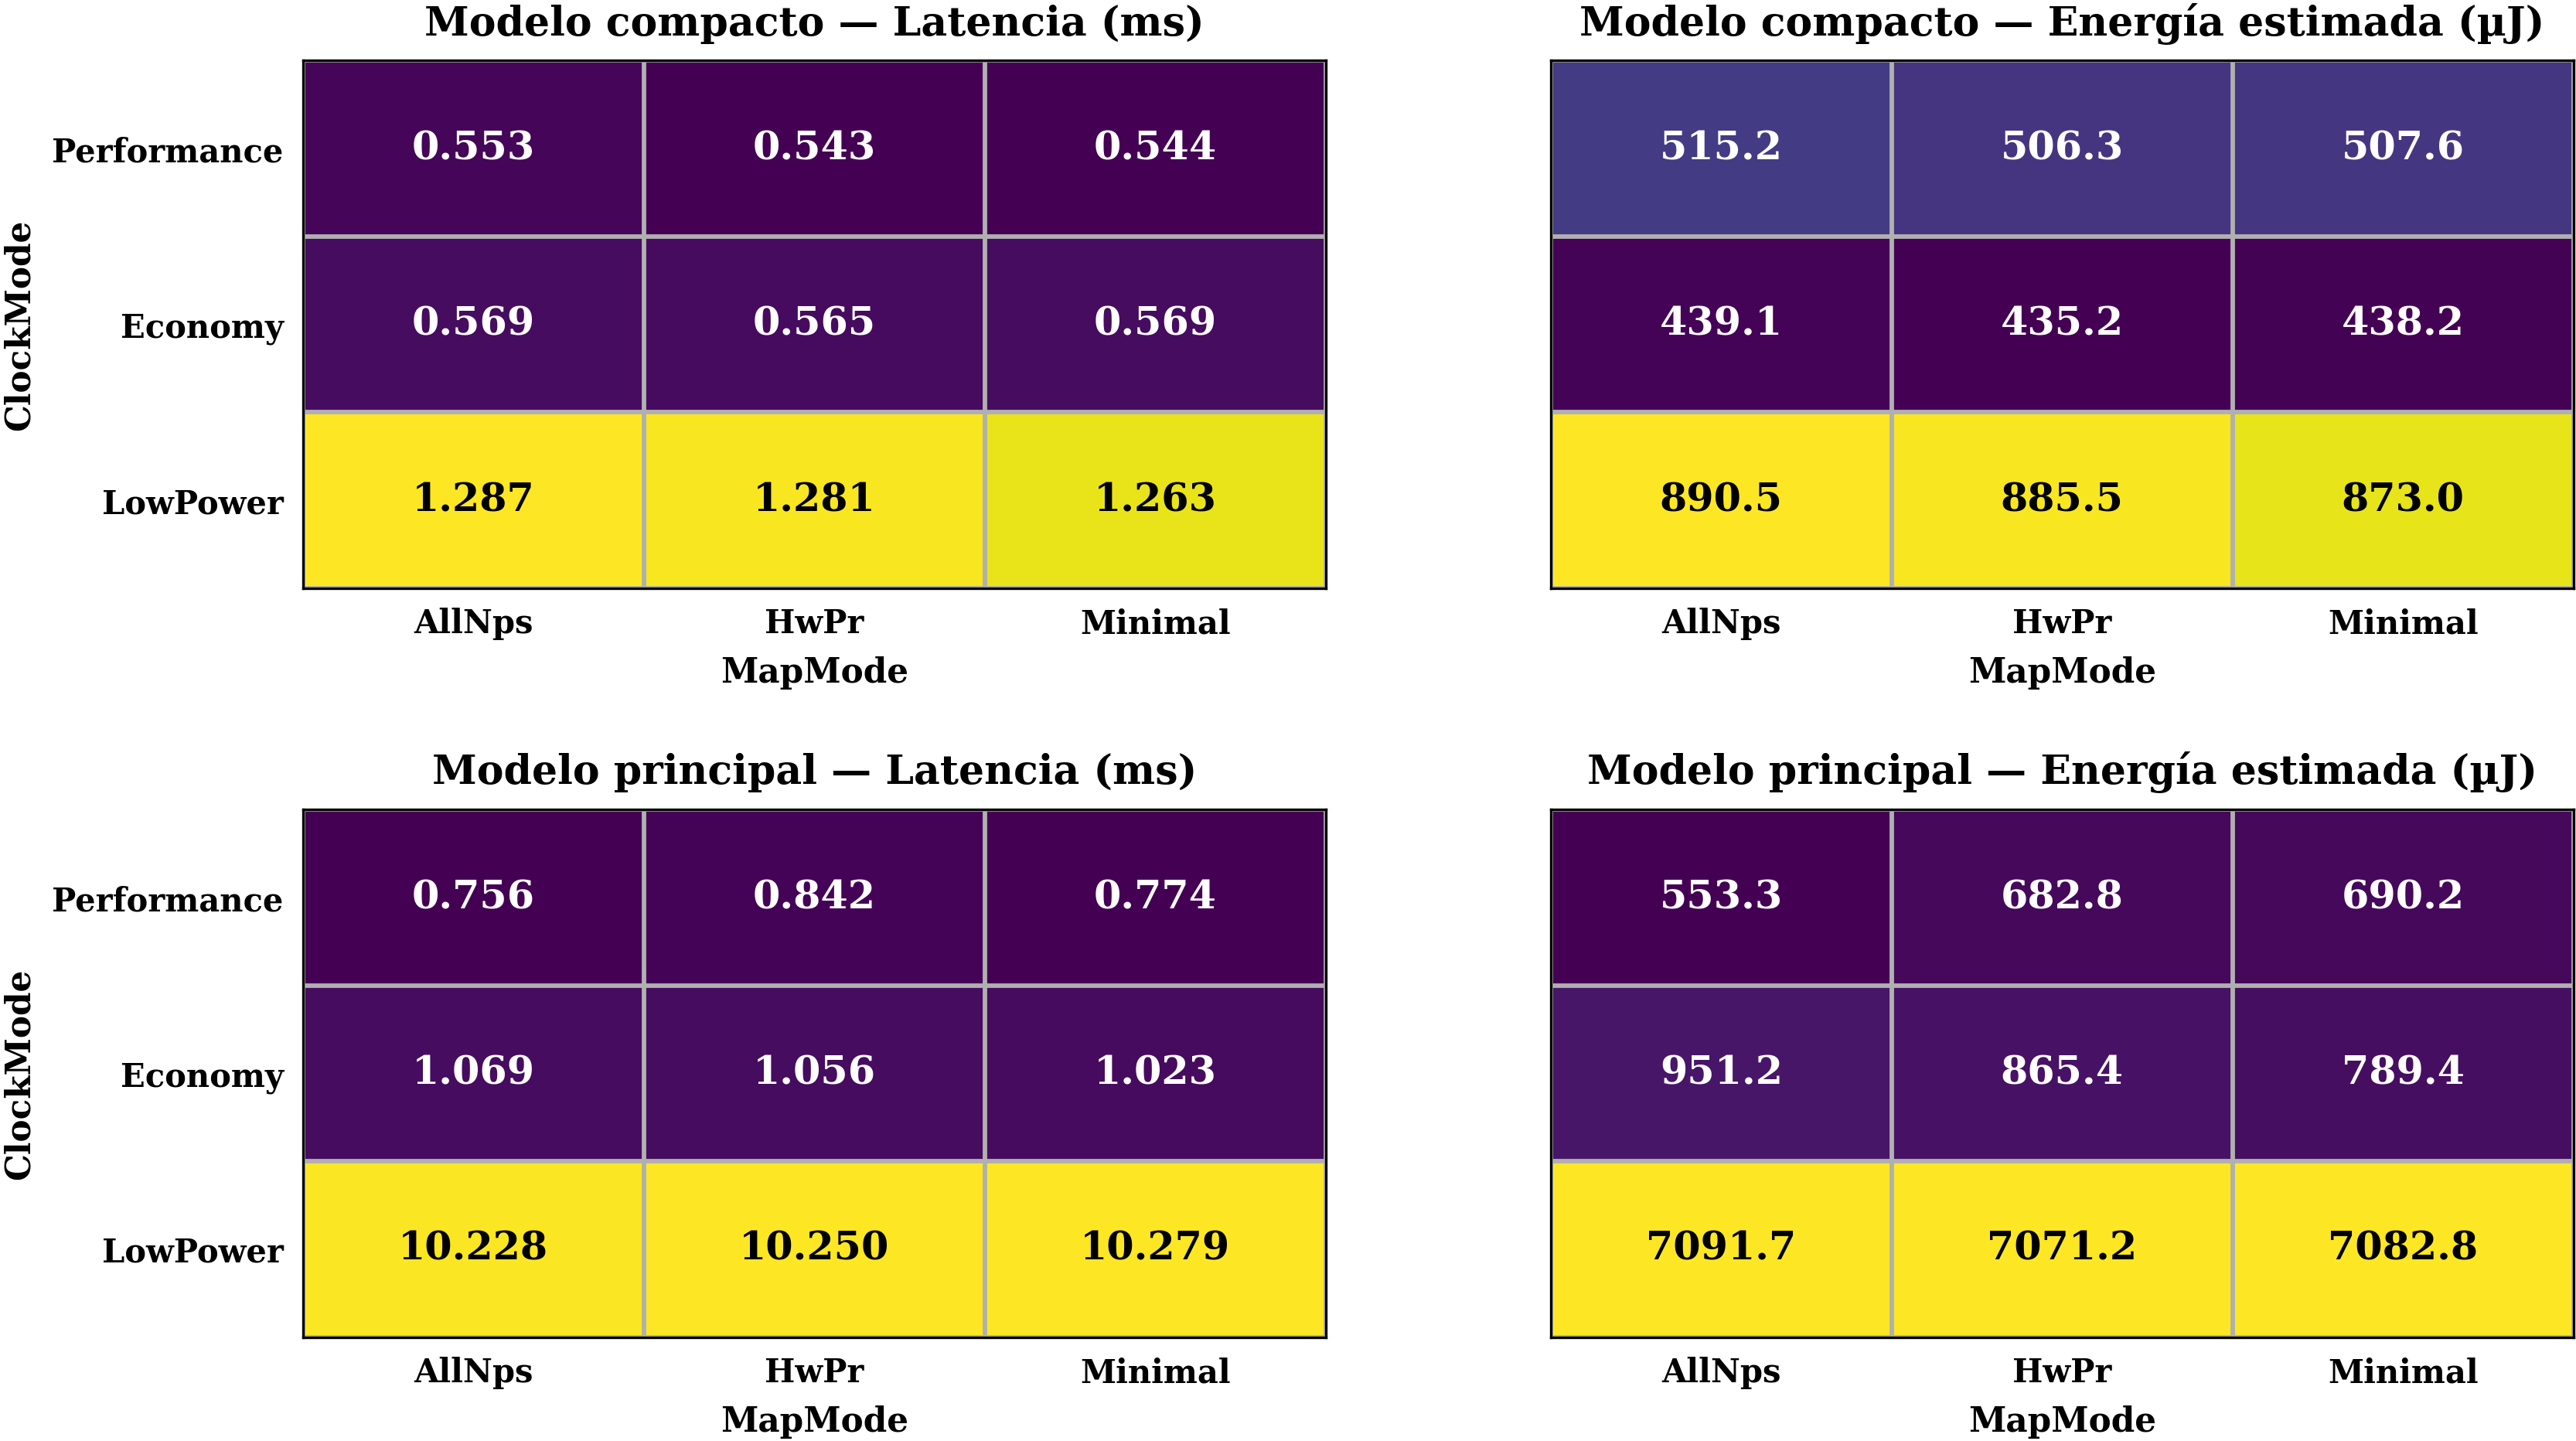
\includegraphics[width=0.88\textwidth]{nine-mode-results.png}
  \caption[Resultados de los modelos AoA]
  {Latencia y energía estimada para los dos modelos en las nueve combinaciones de modo
  de reloj y mapeo evaluadas durante el TFG.}
  \label{fig:tfg-results}
\end{figure}

La latencia se midió desde el host alrededor de la llamada de ejecución. La potencia
corresponde a la medida proporcionada por la API de Akida y no al consumo completo de
la Raspberry Pi, el carrier y la tarjeta.

Estos resultados describen únicamente la plataforma utilizada durante el TFG.
\chapter{Referencia rápida de comandos}
\label{app:comandos}

Este apéndice reúne los comandos principales del procedimiento en Linux.
Las explicaciones y condiciones de uso se encuentran en los capítulos correspondientes.

\section{Comprobar el sistema}

\begin{lstlisting}[language=bash]
uname -r
uname -m
cat /etc/os-release
lspci -nn
\end{lstlisting}

\section{Raspberry Pi 5}

Para un adaptador PCIe no HAT+, edita:

\begin{lstlisting}[language=bash]
sudoedit /boot/firmware/config.txt
\end{lstlisting}

y añade, si todavía no está presente:

\begin{lstlisting}
dtparam=pciex1
\end{lstlisting}

Después reinicia y comprueba la conexión:

\begin{lstlisting}[language=bash]
sudo reboot
lspci -nn
\end{lstlisting}

\section{Controlador PCIe}

En Ubuntu:

\begin{lstlisting}[language=bash]
sudo apt update
sudo apt install dkms build-essential "linux-headers-$(uname -r)"
\end{lstlisting}

Descarga e instala el controlador:

\begin{lstlisting}[language=bash]
git clone https://github.com/Brainchip-Inc/akida_dw_edma.git
cd akida_dw_edma
git rev-parse HEAD
./install.sh
\end{lstlisting}

Comprueba la instalación:

\begin{lstlisting}[language=bash]
dkms status
lsmod | grep -i akida
ls -l /dev/akida*
lspci -nnk
\end{lstlisting}

\section{Entorno de Python}

Desde la carpeta principal del proyecto:

\begin{lstlisting}[language=bash]
python3.11 -m venv .venv
source .venv/bin/activate
python -m pip install --upgrade pip
\end{lstlisting}

Instalación actual de MetaTF:

\begin{lstlisting}[language=bash]
python -m pip install "metatf==2.19.3"
\end{lstlisting}

o entorno de referencia del repositorio:

\begin{lstlisting}[language=bash]
python -m pip install -r requirements/reproducible.txt
\end{lstlisting}

Instala después las herramientas del proyecto:

\begin{lstlisting}[language=bash]
python -m pip install -e . --no-deps
python -m pip check
\end{lstlisting}

\section{Pruebas básicas}

Prueba en software:

\begin{lstlisting}[language=bash]
python examples/00_simulator_smoke.py
akd1000-bringup verify \
  --id smoke \
  --model models/akida_v1_smoke_test.fbz
\end{lstlisting}

Diagnóstico:

\begin{lstlisting}[language=bash]
akd1000-bringup doctor
\end{lstlisting}

Prueba en la tarjeta:

\begin{lstlisting}[language=bash]
akida devices
python examples/01_hardware_smoke.py
\end{lstlisting}

\section{Ejecutar un modelo propio}

\begin{lstlisting}[language=bash]
akd1000-bringup run \
  --model models/model.fbz \
  --input data/input.npy \
  --method forward \
  --clock Performance \
  --map AllNps \
  --output outputs/raw-output.npy
\end{lstlisting}

\section{Benchmark}

\begin{lstlisting}[language=bash]
akd1000-bringup benchmark \
  --model models/model.fbz \
  --input data/inputs.npy \
  --method forward \
  --clock Performance \
  --map AllNps \
  --warmup 8 \
  --repetitions 1 \
  --output outputs/smoke
\end{lstlisting}

\section{Diagnóstico rápido}

\begin{enumerate}
  \item Si la tarjeta no aparece en \code{lspci}, revisa el montaje y la configuración PCIe.
  \item Si aparece en PCIe pero falta \code{/dev/akida*}, revisa el controlador.
  \item Si existe el nodo pero \code{akida.devices()} está vacío, revisa el entorno y los permisos.
  \item Si el modelo de prueba funciona y el modelo propio no, revisa el modelo y sus datos de entrada.
\end{enumerate}
\chapter{Fuentes y limitaciones}
\label{app:fuentes-limitaciones}

Las instrucciones de este manual se basan principalmente en la documentación oficial de
BrainChip, Raspberry Pi y Waveshare, junto con la memoria y los archivos del TFG.

La versión de referencia del entorno utiliza Akida 2.19.1, mientras que la documentación
actual consultada para este manual corresponde a MetaTF 2.19.3. La compatibilidad del
controlador PCIe debe comprobarse antes de utilizar versiones posteriores del kernel o del SDK.

Esta edición todavía no ha sido validada mediante una sesión completa con un usuario nuevo
y acceso físico a la tarjeta. La reproducción del caso AoA requiere además los modelos y
datos originales, que no forman parte de esta entrega.

Las medidas de potencia obtenidas mediante la API de Akida no representan el consumo total
del sistema. El manual tampoco cubre funciones como \emph{edge learning} ni Akida Engine.


\bibliographystyle{plain}
\bibliography{references}
\end{document}
